\documentclass[12pt,oneside]{book} % use larger type; default would be 10pt

\usepackage[utf8]{inputenc} 
\usepackage[czech]{babel}
\usepackage[IL2]{fontenc}
\usepackage[a4paper]{geometry} 
\usepackage[pdftex]{graphicx} 
\usepackage[parfill]{parskip} 		% Activate to begin paragraphs with an empty line rather than an indent
\usepackage[explicit]{titlesec}
\usepackage{titletoc}
\usepackage{multirow}
\usepackage{bytefield}
\usepackage{rotating}
\usepackage{booktabs}  			% for much better looking tables
\usepackage{longtable}
\usepackage{lscape}
\usepackage{array} 	  		% for better arrays (eg matrices) in maths
\usepackage{paralist}  			% very flexible & customisable lists (eg. enumerate/itemize, etc.)
\usepackage{verbatim}  			% adds environment for commenting out blocks of text & for better verbatim
\usepackage{subfig}    			% make it possible to include more than one captioned figure/table in a single float
\usepackage[nottoc,notlof,notlot]{tocbibind} % Put the bibliography in the ToC
\usepackage[titles,subfigure]{tocloft}		 % Alter the style of the Table of Contents
\usepackage{color}
\usepackage[usenames,dvipsnames]{xcolor}
\usepackage{pdfmarginpar}
\usepackage{lastpage}
\usepackage{circuitikz}
\usepackage{tikz}
\usetikzlibrary{shapes,arrows,positioning,snakes,backgrounds,decorations.footprints,shadows,calc,chains} 
\usepackage{wrapfig}
\usepackage{listings}
\usepackage{tabularx}
\usepackage{enumitem}
\usepackage{anyfontsize}
\usepackage[pdftex, colorlinks=true, linkcolor=blue, urlcolor=blue]{hyperref} %should be last

\geometry{papersize={210mm,305mm},total={176mm,260mm}}

\usepackage{fancyhdr} % This should be set AFTER setting up the page geometry

\usepackage[local]{gitinfo2}

\pagestyle{fancyplain}     % options: empty , plain , fancy

\def\projectname{B5: Piano Tales Master}
\def\projectsubname{BROB - Základy robotiky\\[0.5cm]2019}
\def\projectdoc{Dokumentace projektu}

\definecolor{darkgray}{rgb}{0.4,0.4,0.9}
\definecolor{lightdarkgray}{rgb}{0.6,0.6,1.0}

\newcommand{\HRule}{\textcolor{darkgray}{\rule{\linewidth}{2mm}}}

\renewcommand{\headrulewidth}{1mm}
\renewcommand{\footrulewidth}{1mm}
\renewcommand{\plainheadrulewidth}{1mm}
\renewcommand{\plainfootrulewidth}{1mm}

\newcommand{\headrulecolor}{darkgray}
\newcommand{\footrulecolor}{darkgray}

\let\oldheadrule\headrule
\let\oldfootrule\footrule
\def\headrule{\textcolor{\headrulecolor}{\oldheadrule}}
\def\footrule{\textcolor{\footrulecolor}{\oldfootrule}}


\lhead{\projectdoc}
\chead{}
\rhead{\LARGE \projectname}
\lfoot{}
\cfoot{}
\rfoot{\thepage/\pageref{LastPage}}

\voffset 5mm
\setlength\headsep{8mm}

\newcommand{\up}[1]{\begin{sideways}\parbox{15mm}{#1}\end{sideways}}
\newcommand{\bx}[1]{\parbox{0.4\textwidth}{\centering #1}}

\tikzstyle{isipka} = [very thick,fill=none,rounded corners=2mm, color=red!100]
\tikzstyle{iodkaz} = [very thick,fill=none,rounded corners=3mm, color=red!100,line cap=round,align=center]
\tikzstyle{iprvek} = [rectangle, draw=red, rounded corners=3mm, line width=1mm]

\tikzstyle{postup} = [rectangle, draw, rounded corners=3mm, line width=1mm,minimum width=4cm,font=\bf]
\tikzstyle{labl} = [circle, draw, fill=white, rounded corners=3mm, line width=1mm,anchor=east,font=\bf]
\tikzstyle{edg} = [->, line width=1mm]

\tikzstyle{key} = [draw, fill=white, rectangle, rounded corners=2pt, inner sep=4pt, line width=0.5pt, drop shadow={shadow xshift=0.25ex,shadow yshift=-0.25ex,fill=black,opacity=0.75}, font=\scriptsize\sffamily, minimum height=1.5\baselineskip, minimum width=1.5\baselineskip]
\setcounter{secnumdepth}{-1}
\setcounter{tocdepth}{1}

\renewcommand\thepart{\arabic{part}}

\titleformat{\part}
  {\normalfont\normalsize}
  {}
  {20pt}
  {\begin{tikzpicture}[remember picture,overlay]%
	 \fill[lightdarkgray]  (current page.north west) rectangle ([yshift=-13cm]current page.north east);   
	 \node[fill=darkgray, text width=2\paperwidth, rounded corners=6cm, text depth=18cm, anchor=center, inner sep=0pt] at (current page.north east) (parttop) {\strut};
	 \node[anchor=south east, inner sep=0pt,	outer sep=0pt] at ([shift={(-2cm, +1cm)}]parttop.south)  (partnum) {\fontsize{10cm}{10}\selectfont\color{black}\thepart};
	 \node[anchor=north, inner sep=0pt]  at ([yshift=-2pt]partnum.south) (partname) {\large\scshape\bfseries\color{white} ČÁST};
 	 \node[anchor=north east, align=right, inner sep=0pt, outer ysep=2cm] at ([xshift=1cm]partnum.south) {\parbox{.7\textwidth}{\Huge\bfseries\raggedleft\projectname\\#1}};
 	 \node[anchor=north, align=left] at ([yshift=-12.5cm]current page.north) {\parbox{\textwidth}{\startcontents[part]\printcontents[part]{l}{0}{\setcounter{tocdepth}{0}}}};
   \end{tikzpicture}%    
  }

\titleformat{\chapter}
  {\normalfont}%
  {}%
  {20pt}%
  {\begin{tikzpicture}[remember picture,overlay]
    \fill[darkgray] (current page.north west) rectangle ([yshift=-3.5cm]current page.north east);
    \node[anchor=west, align=left, inner xsep=2cm] at ([yshift=-2cm]current page.north west) {\parbox{\textwidth}{\huge\sffamily\bfseries\scshape\color{white}#1}};%
   \end{tikzpicture}%
  }

\titlespacing*{\chapter}{0pt}{50pt}{-70pt}




\begin{document}
	
\begin{titlepage}
    \begin{center}

	~\\[0.5cm]
       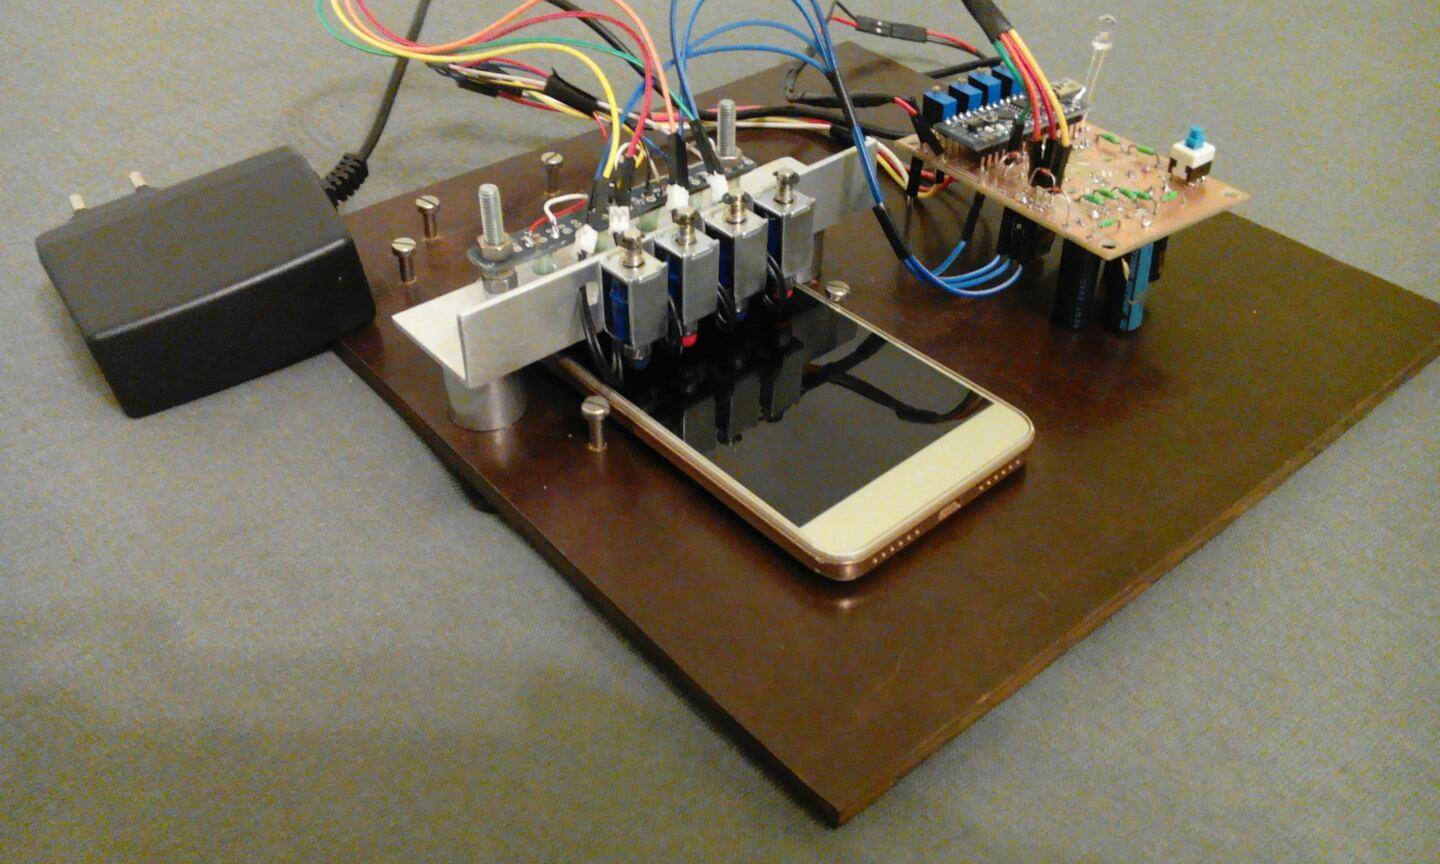
\includegraphics[width=0.85\textwidth]{./img/uvodka.jpg}\\[0cm] 

	~\\[2cm]

    % Title
    \HRule \\[0.4cm]
    { \huge \bfseries \projectname}\\[0.4cm]
       \textsc{\LARGE \projectsubname}\\[0.4cm]
    \HRule \\[1cm]
    
    \textsc{\LARGE \projectdoc}\\[0.5cm]
    \texttt{\Large \gitFirstTagDescribe}\\[1.5cm]

    % Author and supervisor
    \begin{minipage}{0.5\textwidth}
      \begin{center} \large
        
\includegraphics[width=0.85\textwidth]{./img/loga/vut.png}\\[1cm] 
		 \Large\bfseries UAMT FEKT VUT		
      \end{center}
    \end{minipage}%
    \begin{minipage}{0.5\textwidth}\raggedleft\Large\bfseries
 	Lukáš Zezula\par
        Dominik Řičánek\par
    \raggedright    
        Vedoucí projektu: \par
   \raggedleft     
        ing.Adam Ligocki
    \end{minipage}
    \vfill
   \end{center}
\end{titlepage}

\tableofcontents

%%%%%%%%%%%%%%%%%%%%%%%%%%%%%%%%%%%%%%%%%%%%%%%%%%%%%%%%%%%%%%%%%%%%%%%%%%%%%%%%%
%%%%%%%%%%%%%%%%%%%%%%%%%%%%%%%%%%%%%%%%%%%%%%%%%%%%%%%%%%%%%%%%%%%%%%%%%%%%%%%%%
%%%%%%%%%%%%%%%%%%%%%%%%%%%%%%%%%%%%%%%%%%%%%%%%%%%%%%%%%%%%%%%%%%%%%%%%%%%%%%%%%
%%%%%%%%%%%%%%%%%%%%%%%%%%%%%%%%%%%%%%%%%%%%%%%%%%%%%%%%%%%%%%%%%%%%%%%%%%%%%%%%%
\chapter{Analýza zadání}\label{analyza-zadani}
\section{Zadání}
\qquad Vytvořte robota, který bude hrát Piano Tales. Navrhněte stroj, který pomocí Vámi zvoleného HW (snímače a výpočetní jednotky a motorků) bude schopen hrát a porazit člověka ve hře Piano Tales. Referenčním výsledkem bude https://www.youtube.com/watch?v=fqOW84ZTL7k který se pokusíme porazit. Na závěr vznikne krátké propagační video na youtube obsahujcí logo VUT.
Projekt bude veden pomoci GITu. Dokumentace bude vytvořená v LaTeXu. 
\section{Úvod}\label{uvod}
\qquad Cílem projektu, jak je patrno ze zadání, bylo realizovat robota, který by hrál hru Piano Tales a dosahoval lepších výsledků než člověk a ideálně se přiblížil, nebo dokonce překonal referenční výsledek.

\qquad Hra Piano Tales funguje tak, že po obrazovce ve čtyřech lajnách jezdí obdélníky, jejichž stisknutím se zvýší skóre a rychlost s jakou se pohybují. Hra se tedy neustále ztěžuje. Jakmile nezachytíte již zmiňovaný obdélník nebo kliknete mimo jeho plochu, hra končí. Krom těchto obdélníků, které mají pevně definované rozměry, jezdí po obrazovce i delší obdélníkové úseky, které mají stálou šířku, ale jejich délka se různí (viz. Obrázek \ref{pianotales}). Tyto úseky se liší i barevně. Zatímco obdélníky jsou vždy striktně černé, tak barva úseků se mění od černé na začátku úseku po světlejší odstíny modré na konci. Přidržením těchto úseků od počátku do konce se skóre zvýší více než při pouhém stisknutí. 

\begin{figure}[h] \large\centering
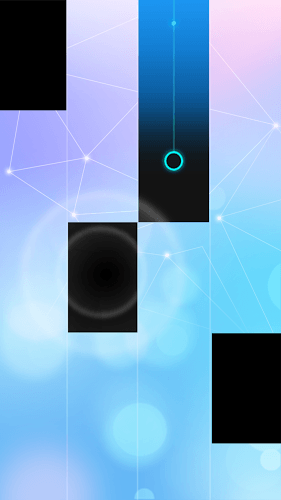
\includegraphics[width=0.30\textwidth]{./img/pianotales.png}\\[1cm] 
\caption{Ukázka hrací plochy hry Piano Tales}
\label{pianotales}
\end{figure}   
      
\section{Nástin řešení}\label{nastin}
\qquad Oproti videu, přiloženému k zadání, jsme neměli k dispozici tablet, kolem kterého by se dali pohodlně rozmístit servomotory, a proto jsme museli použít smartphone, který má podstatně menší rozměry. Toto vedlo na nutnost pracovat s menšími prvky, které by ovládaly dotykový display a složitější mechanickou konstrukci.

\qquad Nejvhodnější se ukázalo být použití elektromagnetů, konkrétně push type solenoidů, které byly pomocí mechanické konstrukce umístěny nad smartphonem tak, aby po přivedení napětí na řídící obvod stiskly specifické místo na dotykovém displayi.

\qquad Ke snímání průběhů obdélníků byly použiti fotorezistory. Tyto byly umístěny dostatečně blízko displaye a ve speciálně vytvořeném pouzdru, aby se minimalizoval vliv okolního osvětlení. 

\qquad Zjednodušený princip, s jakým výsledný robot hraje hru lze vidět na Obrázku \ref{blok_0}. Obdélník, mající černou barvu, se pohybuje po světle modrém pozadí kolem fotorezistoru. To zapříčiní změnu odporu, kterou zachycuje mikroprocesor a měří čas mezi přechody modrá-černá, černá-modrá. Z tohoto času a známých rozměrů obdélníku se vypočte rychlost, s kterou se obdélník pohybuje. Po započítání dopravního zpoždění, které je dáno zejména časem potřebným k sepnutí solenoidu, se určí okamžik, kdy přesně má být přiveden z mikroprocesoru spínací signál na vstup řídícího obvodu.

\begin{figure}[h] \large\centering
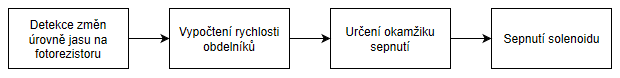
\includegraphics[width=0.80\textwidth]{./img/blok_0.png}\\[1cm] 
\caption{Zjednodušený princip funkce robotu}
\label{blok_0}
\end{figure}   
%%%%%%%%%%%%%%%%%%%%%%%%%%%%%%%%%%%%%%%%%%%%%%%%%%%%%%%%%%%%%%%%%%%%%%%%%%%%%%%%%
%%%%%%%%%%%%%%%%%%%%%%%%%%%%%%%%%%%%%%%%%%%%%%%%%%%%%%%%%%%%%%%%%%%%%%%%%%%%%%%%%
%%%%%%%%%%%%%%%%%%%%%%%%%%%%%%%%%%%%%%%%%%%%%%%%%%%%%%%%%%%%%%%%%%%%%%%%%%%%%%%%%
%%%%%%%%%%%%%%%%%%%%%%%%%%%%%%%%%%%%%%%%%%%%%%%%%%%%%%%%%%%%%%%%%%%%%%%%%%%%%%%%%
\part{MECHANICKÁ ČÁST}\label{mechanika}
\chapter{Návrh v prostředí AutoCAD}\label{CAD}

\begin{figure}[h]\large\centering
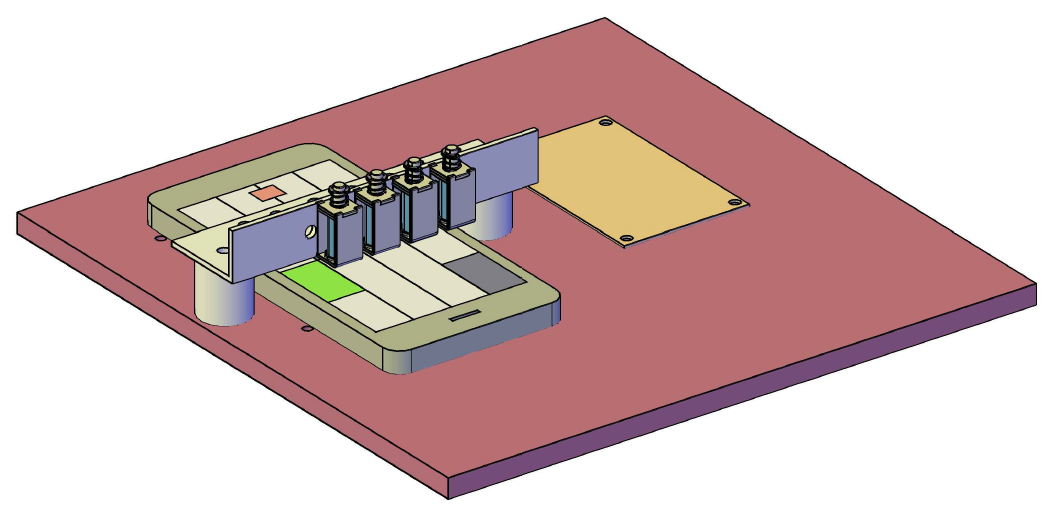
\includegraphics[width=1.00\textwidth]{./img/mech_cad0.png}\\[1cm] 
\caption{Model mechanické části v prostředí AutoCAD jiho-západní pohled}
\label{mech_cad0}
\end{figure}  

\begin{figure}[h]\large\centering
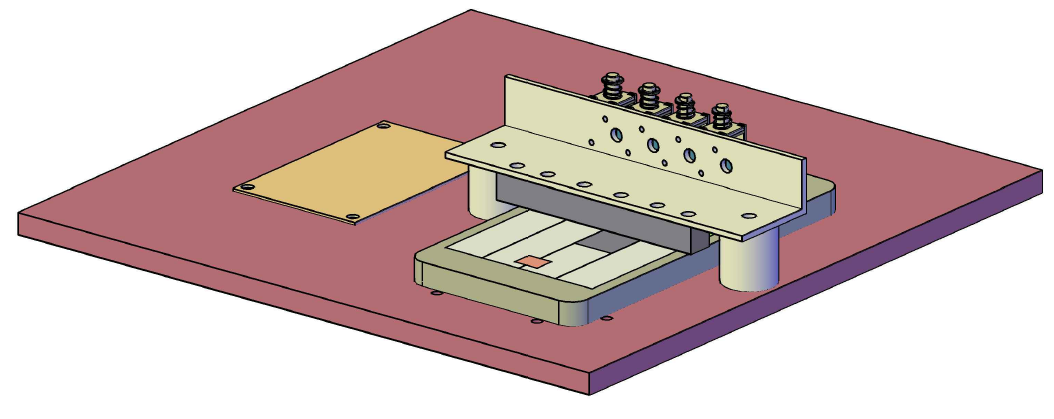
\includegraphics[width=1.00\textwidth]{./img/mech_cad1.png}\\[1cm] 
\caption{Model mechanické části v prostředí AutoCAD severo-západní pohled}
\label{mech_cad1}
\end{figure}  

\pagebreak

\section{Popis částí modelu}\label{mech_casti}
\qquad Model byl pomyslně rozdělen na 5 částí. Konkrétně se jedná o podstavu, L-profil, válcové spojky, pouzdro na fotorezistory a solenoidy. Tyto části jsou navrženy tak, aby byly demontovatelné (spoje jsou realizovány pouze šrouby a případně maticemi). Jak na sebe jednotlivé části navazují můžeme vidět na Obrázku \ref{mech_cad0} a \ref{mech_cad1}. Oranžový obdélníkový profil představuje plošný spoj.
%%%%%%%%%%%%%%%%%%%%%%%%%%%%%%%%%%%%%%%%%%%%%%%%%%%%%%%%%%%%%%%%%%%%%%%%%%%%%%%%%
%%%%%%%%%%%%%%%%%%%%%%%%%%%%%%%%%%%%%%%%%%%%%%%%%%%%%%%%%%%%%%%%%%%%%%%%%%%%%%%%%
%%%%%%%%%%%%%%%%%%%%%%%%%%%%%%%%%%%%%%%%%%%%%%%%%%%%%%%%%%%%%%%%%%%%%%%%%%%%%%%%%
%%%%%%%%%%%%%%%%%%%%%%%%%%%%%%%%%%%%%%%%%%%%%%%%%%%%%%%%%%%%%%%%%%%%%%%%%%%%%%%%%
\part{Návrh a realizace elektronické části}\label{elektro}

\chapter{BLABLA}\label{BLABLA}
\section{2xBLABLA}\label{2xBLABLA}

%%%%%%%%%%%%%%%%%%%%%%%%%%%%%%%%%%%%%%%%%%%%%%%%%%%%%%%%%%%%%%%%%%%%%%%%%%%%%%%%%
%%%%%%%%%%%%%%%%%%%%%%%%%%%%%%%%%%%%%%%%%%%%%%%%%%%%%%%%%%%%%%%%%%%%%%%%%%%%%%%%%
%%%%%%%%%%%%%%%%%%%%%%%%%%%%%%%%%%%%%%%%%%%%%%%%%%%%%%%%%%%%%%%%%%%%%%%%%%%%%%%%%
%%%%%%%%%%%%%%%%%%%%%%%%%%%%%%%%%%%%%%%%%%%%%%%%%%%%%%%%%%%%%%%%%%%%%%%%%%%%%%%%%
\part{Programová část}\label{program}

\chapter{BLABLA}\label{BLABLA}
\section{2xBLABLA}\label{2xBLABLA}

%%%%%%%%%%%%%%%%%%%%%%%%%%%%%%%%%%%%%%%%%%%%%%%%%%%%%%%%%%%%%%%%%%%%%%%%%%%%%%%%%
%%%%%%%%%%%%%%%%%%%%%%%%%%%%%%%%%%%%%%%%%%%%%%%%%%%%%%%%%%%%%%%%%%%%%%%%%%%%%%%%%
%%%%%%%%%%%%%%%%%%%%%%%%%%%%%%%%%%%%%%%%%%%%%%%%%%%%%%%%%%%%%%%%%%%%%%%%%%%%%%%%%
%%%%%%%%%%%%%%%%%%%%%%%%%%%%%%%%%%%%%%%%%%%%%%%%%%%%%%%%%%%%%%%%%%%%%%%%%%%%%%%%%
\part{Shrnutí a závěr}\label{shrnuti}

%%%%%%%%%%%%%%%%%%%%%%%%%%%%%%%%%%%%%%%%%%%%%%%%%%%%%%%%%%%%%%%%%%%%%%%%%%%%%%%%%
%%%%%%%%%%%%%%%%%%%%%%%%%%%%%%%%%%%%%%%%%%%%%%%%%%%%%%%%%%%%%%%%%%%%%%%%%%%%%%%%%
%%%%%%%%%%%%%%%%%%%%%%%%%%%%%%%%%%%%%%%%%%%%%%%%%%%%%%%%%%%%%%%%%%%%%%%%%%%%%%%%%
%%%%%%%%%%%%%%%%%%%%%%%%%%%%%%%%%%%%%%%%%%%%%%%%%%%%%%%%%%%%%%%%%%%%%%%%%%%%%%%%%
\part{Literatura}\label{literatura}

\end{document}
